\documentclass[12pt]{article}
\usepackage[utf8]{inputenc}
\usepackage[spanish,mexico]{babel}
\usepackage{float}

\usepackage{graphicx}
\graphicspath{{images/}}

\usepackage{vmargin}
\setmarginsrb{3 cm}{2.5 cm}{3 cm}{2.5 cm}{1 cm}{1.5 cm}{1 cm}{1.5 cm}

\begin{document}

\title{Actividad 1: Preparando documentos científicos con LATEX}
\author{Martin Alejandro Paredes Sosa}
\date{Enero 2016}
\maketitle

\section{Péndulo Simple}
Es una idealización de un ``péndulo real" pero aislado utilizando las siguinetes supuestos:
\begin{itemize}
\item El cable o cuerda del péndulo se considera sin masa, no esxtendible y siempre tensa.
\item Es considerada una masa puntua.l %Checar traducción
\item El movimiento es bidimensional(sos direcciones) y sigue al movimiento de un arco.
\item EL movimiento no pierde energia contra la fricción a o resistencia al aire.
\item El campo gravitacional es uniforme.
\item El soporte no se mueve.
\end{itemize}

La ecuación diferencial que representa el movimento del pédulo es la siguiente:
\begin{equation}
\frac{d^2\theta}{dt^2}+\frac{g}{l}\sin\theta=0
\end{equation}
donde $g$ es la acerelación debida a la gravedad, $l$ la longitud del péndulo y $\theta$ es el ángulo de desplazamiento.

%\subsection{Derivación de ``Fuerza" de la ecuación 1}
%Usando como referencia a la Figura 1, que muestra las fuerazas que actuan sobre el péndulo. el camino que recorre el péndulo es un arco. El ángulo $\theta$ se mide en radianes lo cual es crucial. La flecha azul representa la fuerza gravitacional, las flechas moradas son la misma fuerza nomas que descompuetas en sus diferentes compentes paralelas y perpendiculares al movimiento en el instante. La direccion de la velociadad instantanea siempre es sobre el eje rojo
%\begin{figure}[H]
%\centering
%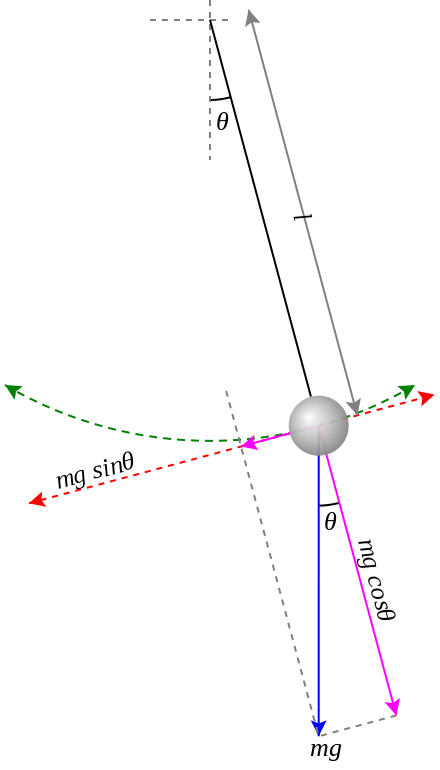
\includegraphics[width=4cm]{pendulo}
%\caption{Diagrama de fuerzas del péndulo simple}
%\end{figure}

\end{document}